%% This is an example first chapter.  You should put chapter/appendix that you
%% write into a separate file, and add a line \include{yourfilename} to
%% main.tex, where `yourfilename.tex' is the name of the chapter/appendix file.
%% You can process specific files by typing their names in at the 
%% \files=
%% prompt when you run the file main.tex through LaTeX.
\chapter{Final Implementation}
This chapter describes the final implementation of the entire OMR/MIDI musical stream alignment and correction system. First there will be an overview of the entire system. Then, there will be discussion on the final implementation of each of the large modules that is divorced from the context of the \texttt{OMRMIDICorrector} class. Afterwards, I will present an example use case of the system. I will conclude with a discussion of design tradeoffs and choices that I made in implementing the system.

The final implementation of the OMR/MIDI musical stream alignment and correction system. can be found in \texttt{omrMidiCorrector.py}. The OMR system is a combination of one or more of each of the \texttt{Hasher}, \texttt{Aligner}, and \texttt{Fixer} modules with specific parameters set. 

The inputs to the system are two \texttt{music21} streams (one OMR, one MIDI). The output of the system is a corrected OMR stream. 

\section{OMRMIDICorrector}

\subsection{System Overview}
The system is the \texttt{OMRMIDICorrector} class in \texttt{omrMidiCorrector.py}. This class is initialized with a \texttt{midiStream}, an \texttt{omrStream} and an optional \texttt{Hasher}. The \texttt{Hasher} parameter is optional because the system provides a default \texttt{Hasher} with some all-purpose settings if no \texttt{Hasher} is passed in. The method \texttt{processRunner} is the main method of this class that preprocesses the streams, sets up the appropriate \texttt{Hasher}, and calls the aligning and fixing methods.

\begin{figure}[!h]
\centering
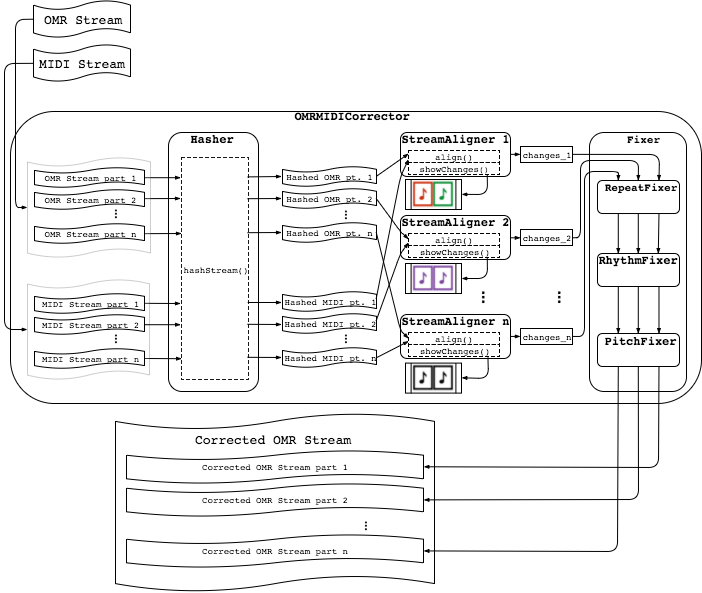
\includegraphics[width=\textwidth]{sysdiag10}
\caption[System diagram.] {The inputs to the system are OMR and MIDI streams. The output of the system is a corrected OMR stream.}
\end{figure}

\subsubsection{processRunner: preprocessStreams}\label{processrunner1}
The \texttt{processRunner} first verifies the streams that are passed in and preprocess them before being hashed, aligned, and fixed in the method \texttt{preprocessStreams}

The first thing that \texttt{preprocessStreams} does is discretize the parts of the stream if the user has set \texttt{discretizeParts} to be \texttt{True}. Discretizing parts means to split the input streams into their constituent parts, so that the input streams are aligned part-wise. Since music is often comprised of multiple parts, this preprocessing step allows for input streams that contain nested streams. Take for example, an OMR/MIDI alignment of a string quartet. Both the OMR and MIDI inputs are stream in and of themselves, and so are all individual instrumental parts within both of the streams. 

A good alignment of the piece would involve aligning corresponding instrumental parts with each other to ensure that the beginnings and ends of corresponding parts aligned with each other. However, if we treat the inputs both as one long stream composed of four serial streams instead of four parallel streams, only the beginnings of the first instrumental parts and the ends of the last instrumental parts would be guaranteed to be aligned with each other. This guarantee comes from the global alignment method that I chose to implement. The figures below illustrate the phenomenon. 

\begin{figure}[!h]
\centering
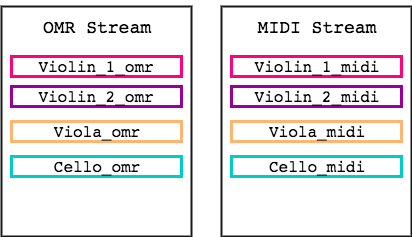
\includegraphics[width=.5\textwidth]{omrmidisheets2}
\caption{An example string quartet stream and its four parts.}
\vspace{10mm}
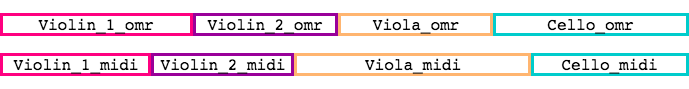
\includegraphics[width=.9\textwidth]{badalignstream2}
\caption[A bad alignment setup] {A bad alignment setup of the quartet would treat the entire piece as four serial streams and only the only guaranteed alignment would be between the beginning of the first part and the end of the last part.}
\vspace{10mm}
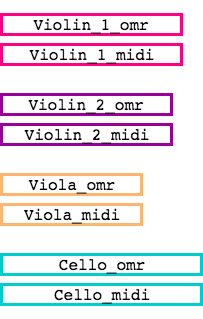
\includegraphics[width=.25\textwidth]{goodalignstream}
\caption[A better alignment setup] {A better alignment setup of the quartet would do part-wise alignment instead of treating the entire piece as a sequence of parts. This methodology guarantees that the beginnings and ends of each part are aligned.}
\end{figure}

By default, \texttt{discretizeParts} is set to \texttt{True}. However, the user ultimately has the choice to align input streams part-wise or After a stream is split up into its constituent parts, the parts are stored in the lists \texttt{midiParts} and \texttt{omrParts}. The aligners and fixers work on all of the elements in the list, and so the entire system is agnostic to the number of parts; a stream comprised of a single part is processed in the same way as a multi-instrumental score. 

Then, \texttt{preprocessStreams} checks if the number of parts in MIDI and the OMR stream are the same. If they are off by more than one, then a \texttt{OMRMIDICorrectorException} is raised and the process halts. This is a cursory check to see if the two input streams can even reasonably be aligned.

If the numbers of parts are off by exactly one, then \texttt{preprocessStreams} spins up a lightweight \texttt{StreamAligner} object to try and see if there is an implicit bassline, where the bass doubles the cello part but an octave lower. In such a scenario, the OMR score would have one fewer part than the MIDI score because a bassist would read the cello line while reading sheet music, but the MIDI score would explicitly list all the instrument lines. If the similarity of the two streams is above a certain threshold, then I conclude that that bass part doubles the cello part and we disregard it in the alignment process. The \texttt{checkBassDoublesCello} method and its use of an \texttt{StreamAligner} object to determine whether two streams are an octave apart is a incidental example of a different use case of the \texttt{StreamAligner}.

\subsubsection{processRunner: setupHasher} \label{setuphasher}
The next step in the \texttt{processRunner} method is setting up the \texttt{Hasher} object that will be used to hash both input streams. This is done in the \texttt{setupHasher} method. If user has passed in a \texttt{Hasher} object upon instantiation of an \texttt{OMRMIDICorrector} object, then that is used. Otherwise this method sets up a default \texttt{Hasher} with settings we have found to be generally effective in the \texttt{setDefaultHasher} method. The default \texttt{Hasher} hashes only pitch and duration and includes references to the original stream elements. 

\subsubsection{processRunner: alignStreams}
This method creates a \texttt{StreamAligner} object for each pairwise MIDI part and OMR part found in \texttt{midiParts} and \texttt{omrParts} and aligns the two parts, calculates their similarity metrics, and visually shows the changes and alignment if \texttt{debugShow} is \texttt{True}. There is more detail about how the \texttt{StreamAligner} object works in section \ref{aligner}

\subsubsection{processRunner: fixStreams}\label{processrunner2}
The last step is of the entire process is to fix the OMR stream. While the \texttt{Fixer} still remains in development, the description of this method and the \texttt{Fixer} in section \ref{fixer} will remain at a high level. 

In its final implementation, \texttt{fixStreams} should create instances of the \texttt{OMRMidiFixer} object, one per pair of aligned streams and their \texttt{changes} list. This is the base class that all other \texttt{Fixer} objects inherit from. The user would be able to choose which \texttt{Fixer} objects they want to create and use on all the pairs of streams. 

Currently, in order to use the two available child \texttt{Fixer} objects, a user can manually create \texttt{OMRMidiFixer} and \texttt{DeleteFixer} and/or \texttt{EnharmonicFixer} objects using the \texttt{changes} lists that \texttt{processRunner} creates.

\section{Hasher}
The \texttt{Hasher} object used in the final implementation is a specific instance of the \texttt{Hasher} object described in section \ref{hasher}. The user can choose to pass in their own instance of \texttt{Hasher} or use the default \texttt{Hasher} provided.

\subsection{The Default Hasher}
The default \texttt{Hasher}, as described in section \ref{setuphasher}, hashes only pitch and duration of stream elements and set \texttt{includeReference} to be \texttt{True}. This setting is general enough to provide for a reasonable alignment for most generic alignment problems. But for more niche problems (for example, a rhythmic alignment), the user ought to define their own \texttt{Hasher} and the default \texttt{Hasher} should not be used. 

\subsection{NoteHashWithReference}
One update I made to the original \texttt{Hasher} was the addition of a new type of \texttt{NamedTuple} that includes a reference to the original element that is hashed and stored within the tuple. This new type provided access to the original stream elements which was necessary for three reasons:
\begin{enumerate}
\item It allows the user to visually see the alignment using the \texttt{showChanges} method in the \texttt{Aligner}. A list of the changes between two streams can be hard to parse and see patterns within, so this method provides a more visually appealing way of interpreting the list of changes.
\item It allows the user to access other elements in the context of the original stream element. For example, it might be helpful to be able to access the most recent key signature change in the stream for some fixing purpose. 
\item In order for the \texttt{Fixer} to fix the OMR stream, it must be able to change the original elements. 
\end{enumerate}

\section{Aligner} \label{aligner}
\subsection{System Overview}
\texttt{Aligner.py} contains the \texttt{StreamAligner} class that is the engine of the Alignment step. \texttt{StreamAligner} accepts as input two \texttt{music21} streams, one specified as a source stream, one as a target stream. The main functionality of \texttt{StreamAligner} is that it produces a global alignment between the source and the target streams in the form of a list of Change Tuples that maps each element in the source stream to an element in the target stream via one of the four change operations (insertion, deletion, substitution, no change). Additionally, \texttt{StreamAligner} also outputs a basic measurement of similarity between the two stream inputs \texttt{similarityScore}. Lastly \texttt{StreamAligner} has a \texttt{show} function that visually displays the alignment between the source and target streams. 

\subsection{Producing a Global Alignment}
The main objective of the Aligner is to produce a global alignment of two streams. In order to do so, it must hash the two streams with an instance of a \texttt{Hasher} (either passed in as a parameter during instantiation of a \texttt{StreamAligner} or using a default Hasher built into the \texttt{StreamAligner} class). After the two streams are hashed, \texttt{StreamAligner} sets up a distance matrix, a la the method described in Chapter 2 for classic string alignment, populates the matrix, and then performs a backtrace of the matrix starting the lower right corner to produce the alignment.

\subsubsection{Pre-Alignment: Setting Appropriate Parameters}
In the interest of being a modular system, I chose to give the programmer the option of setting their own Hasher. Upon instantiation of a \texttt{StreamAligner}, the programmer can choose to pass in an instance of a Hasher. If no Hasher is set initially, then \texttt{StreamAligner} uses the default Hasher that is set to hash Notes, Rests, and Chords, and their MIDI pitches and durations. The default Hasher is generic enough to be able to work with general alignment, but a more niche problem would require the programmer to use a Hasher more specific to their problem

I also chose to leave the cost of Insertion, Deletion, and Substitution easily substitutable as well. By default, the cost of both Insertion and Deletion is equal to the length of one of the \texttt{NoteHashWithReference} tuples, which is exactly the number of properties that are hashed of any musical element. (So in the case of the default Hasher, Insertion and Deletion both have cost 2.) The cost of Substitution between two \texttt{NoteHashWithReference} tuples is equal to the number of properties they don't have in common with each other. For example, the cost of substituting 
$$ \texttt{NoteHashWithReference(pitch=59, offset=1.0, duration=2.0)} $$
with either 
$$\texttt{NoteHashWithReference(pitch=59, offset=1.0, duration=3.0)} $$ or 
$$\texttt{NoteHashWithReference(pitch=60, offset=1.0, duration=2.0)} $$
would have a cost of 1. 

\subsubsection{Pre-Alignment: Hashing the Streams}
The alignment algorithm can only be applied after the streams are represented in a hashed format as a list of \texttt{NoteHashWithReference} tuples. Both input streams will be hashed and stored as the \texttt{hashedTargetStream} and the \texttt{hashedSourceStream}. The hashed format is the analog to a string and each \texttt{NoteHashWithReference} tuple is the analog to a character in classic string alignment.

It recommended that the hasher used to the hash the streams be set to include references to the original stream by using \texttt{NoteHashWithReference} tuples in the creation of the hash (as opposed to the \texttt{NoteHash} tuple that has much less overhead), and in the default hasher,  This ensures that the \texttt{show} function and future fixers have access to the original objects that each hash came from. This makes it easier to color the original objects in the case of the show function and to extract any necessary metadata that wasn't encoded in the hash for future fixers.

There is also an option to indicate that the streams passed in are already hashed, but in the context of my thesis work, this should never be the case. 

\subsubsection{Alignment: Initializing the Distance Matrix}
The first step in the alignment process is initializing the distance matrix. We set up an empty $n+1 \times m+1$ matrix, where $n$ is the length of the hashed target stream and the $m$ is the length of the hashed source. The extra column and extra row are populated with initial costs that correspond to just Insertion or just Deletion operations. In the leftmost column, the value $i \times insertCost$ is put into entries $(i, 0)$. In the topmost row, the value $j \times deleteCost$ is put into entries $(0, j)$. 

\subsubsection{Alignment: Populating the Distance Matrix}
The next step in the alignment process is to fill in the remainder of the distance matrix with values generated with these update rules. 

\begin{equation*}
\begin{split}
\text{D[i][j]} = &  \text{min \{ }\\
& \text{D[i-1][j] + insCost,} \\
& \text{D[i][j-1] + delCost,} \\
& \text{D[i-1][j-1] + subCost} \\
\text{\}}
\end{split}
\end{equation*}


where 
\begin{align*}
	\text{insCost = }  {}& \text{insertCost(hashedSourceStream[0])} \\
	\text{delCost = } {}& \text{deleteCost(hashedSourceStream[0])} \\ 
	\text{subCost = } {}& \text{substitutionCost(}  \text{hashedTargetStream[i-1]},  \-
	\text{hashedSourceStream[j-1])} \\						
\end{align*}

Each entry A[i][j] in the distance matrix stores the lowest cost for aligning\\
 \texttt{hashedTargetStream[i]} with \texttt{hashedSourceStream[j]}. There are 4 possible ways of relating the two tuples. 
\begin{enumerate}
\item \textit{\texttt{hashedTargetStream[i]} is an insertion} - in the case of insertion, the cost of aligning \texttt{hashedTargetStream[i]} with \texttt{hashedSourceStream[j]} is equal to the cost of aligning \texttt{hashedTargetStream[i-i]} with \texttt{hashedSourceStream[j]} plus the cost of insertion.

\item \textit{\texttt{hashedTargetStream[i]} is a deletion} - similar to the insertion case, for deletion, the cost of aligning \texttt{hashedTargetStream[i]} with \texttt{hashedSourceStream[j]} is equal to the cost of the subproblem of aligning \texttt{hashedTargetStream[i]}  with \texttt{hashedSourceStream[j-i]} plus the cost of deletion.

\item \textit{\texttt{hashedTargetStream[i]} is a substitution of \texttt{hashedSourceStream[j]}} - in the case of substitution, the cost of aligning \texttt{hashedTargetStream[i]} with \texttt{hashedSourceStream[j]} is equal to the cost of the subproblem of aligning \texttt{hashedTargetStream[i-i]} with \texttt{hashedSourceStream[j-1]} plus the cost of a substitution of  \texttt{hashedSourceStream[j]} for \texttt{hashedTargetStream[i]}.
 
\item \textit{No change between the two tuples i.e. the two tuples are the same} - same as above, where substitutionCost(\texttt{hashedTargetStream[i]}, \texttt{hashedSourceStream[j]}) is 0.
\end{enumerate}

The method \texttt{populateDistanceMatrix} fills in all the entries of the distance matrix using the rules and calculations listed above. It is important to note that in my work, all changes are made relative to \texttt{TargetStream}. That is, whenever possible, \texttt{SourceStream} is the stream that is being transformed into \texttt{TargetStream}. This invariant holds because in OMR/MIDI correction, the approach and direction I take is to change OMR into MIDI. Therefore, the MIDI stream is always the \texttt{TargetStream} and the OMR stream is always the \texttt{SourceStream}. It is certainly possible to go in either direction, but this paper will do it this way. 

\subsubsection{Alignment: Backtrace to Find the Best Alignment and Create the Changes List}
Once the distance matrix has been completely filled in, we use a backtrace starting from the bottom right hand corner of the matrix (i.e. A[i][j]) to find the path of least of cost. 

Starting from the value found at A[i][j], we look at the values directly above, to the left, and diagonal in the up-left direction. That is, we look at the values in A[i-][j], A[i][j-1], and A[i-1][j-1]. Among these three values, we choose the minimum value. The combination of direction and value that we moved in tells us what kind of operation was performed to align NoteHashWithReference tuples \texttt{hashedSourceStream[i]} and \texttt{hashedSourceStream[j]}:
\begin{enumerate}
\item if the direction is up, then regardless of the value, this corresponds to an insertion operation.
\item if the direction is left, then regardless of the value, this corresponds to an insertion operation.
\item if the direction is diagonal up-left, and the value at A[i-1][j-1] is \textit{different} from the value at A[i][j], then this corresponds to a substitution operation.
\item if the direction is diagonal up-left, and the value at A[i-1][j-1] is the \textit{same} as the value at A[i][j], then this corresponds to a no-change operation.
\end{enumerate}  

We continue this backtrace until we end up back at A[1][1]. Since we are using a global alignment technique, we should always end up back at this entry. If at the end of backtrace we end up in another part of the distance matrix, the method throws an \texttt{AlignmentException}. 

Additionally, at every step of the backtrace, we create a \texttt{ChangeTuple} that holds references to the original musical elements that are represented in the original \texttt{SourceStream} and \texttt{TargetStream} and the kind of operation (insertion, deletion, substitution, no-change) that links them. Then we insert this \texttt{ChangeTuple} into the beginning of the \texttt{changes} list.

This is all performed in the \texttt{calculateChangesList} method. 

\subsubsection{Post-Alignment: Measures of Similarity}
After the backtrace to find the alignment, there is enough data to calculate some basic metrics of similarity. 

\texttt{changesCount} is a Counter object that provides a count of how many of each of the four different change operations appear in the \texttt{changes} list. 

\texttt{similarityScore} is a float between 0 and 1.0 that is the ratio of \texttt{NoChange} operations to the total number operations in the \texttt{changes} list.
\subsubsection{Post-Alignment: Visual Display of Alignment}
The \texttt{showChanges} method provides a visual display of how the two streams are related via the \texttt{changes} list. For each \texttt{ChangeTuple} in the list, this method goes back to the initial reference and changes the color of the element in reference and adds in an id number as a lyric to that element if the change operation is not a \texttt{NoChange}. The color is determined by the type of change operation. Green corresponds to an insertion, red to deletion, and purple to substitution. The id number is the index of the \texttt{ChangeTuple} in the list. 

The figures below shows the visual display of alignment between the Violin 1 parts of an excerpt of \textit{Eine Kleine Nachtmusik, K.525} by W.A. Mozart. and a MIDI recording of the same piece.
\begin{figure}[H]
\centering
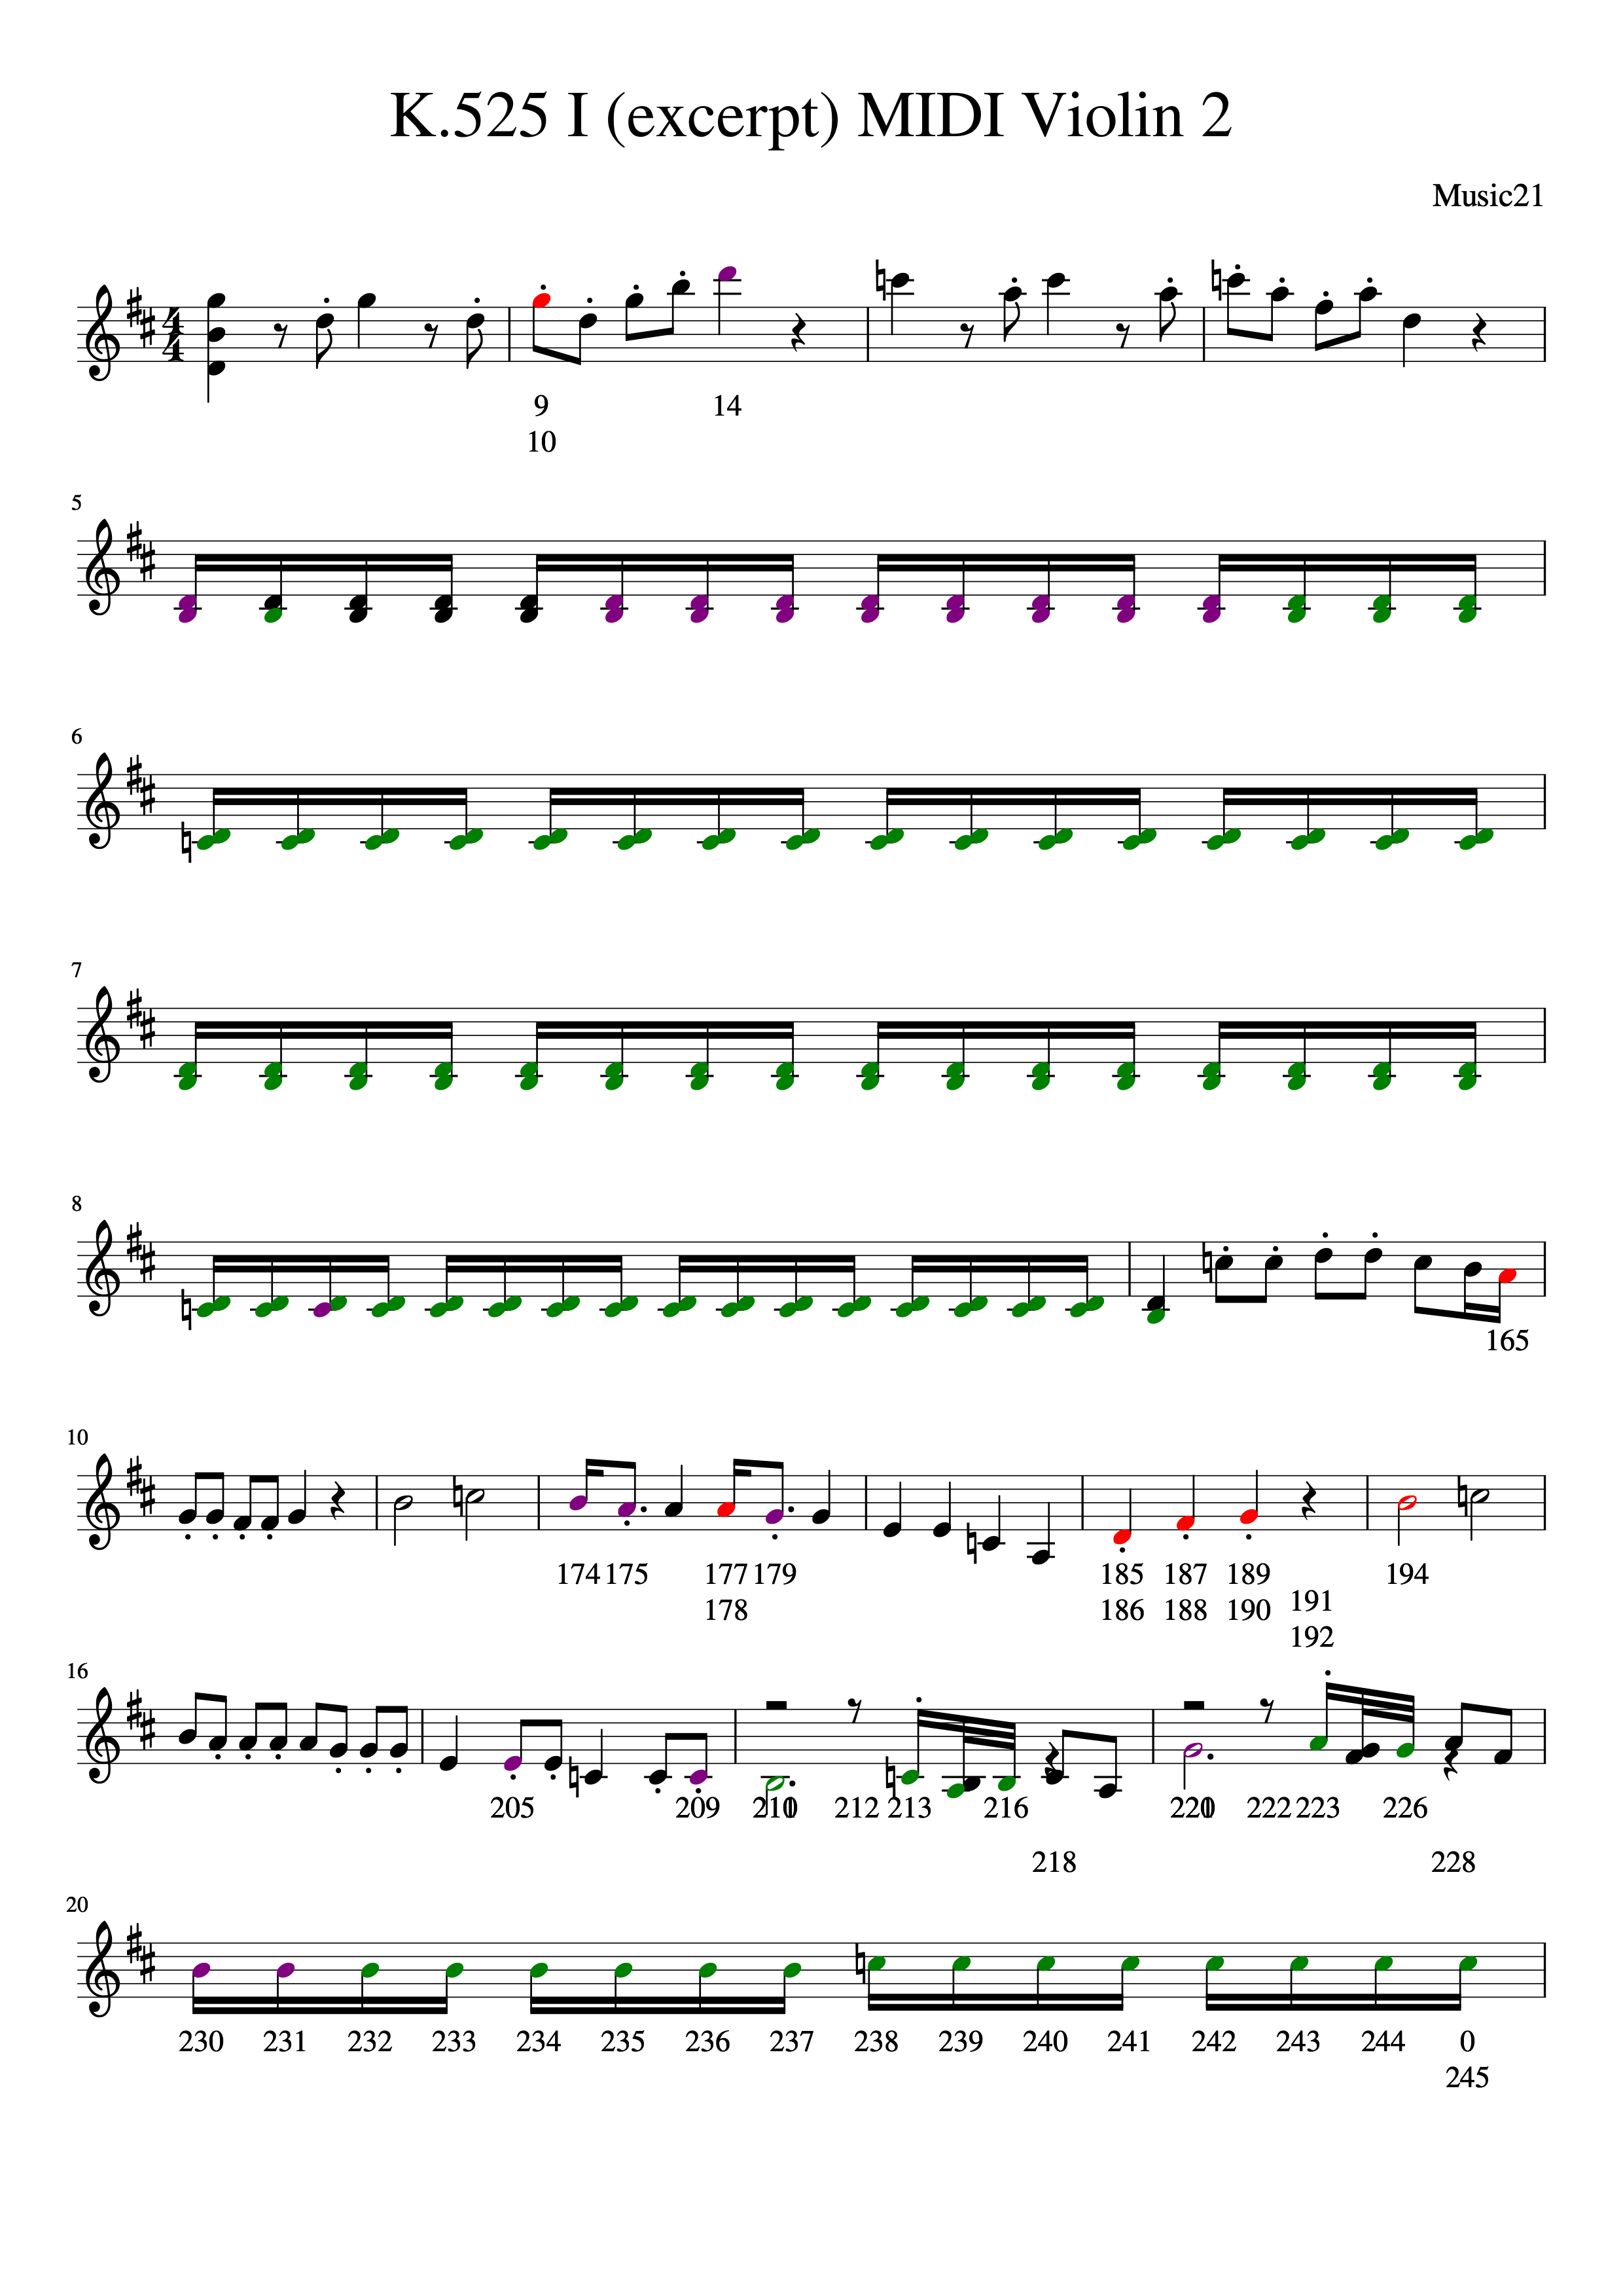
\includegraphics[width =.95\textwidth]{K525_I_MIDI_Violin_2-1}
\caption{Visual display of changes in the Violin 1 part of target (MIDI) stream.}
\end{figure}

\begin{figure}[H]
\centering
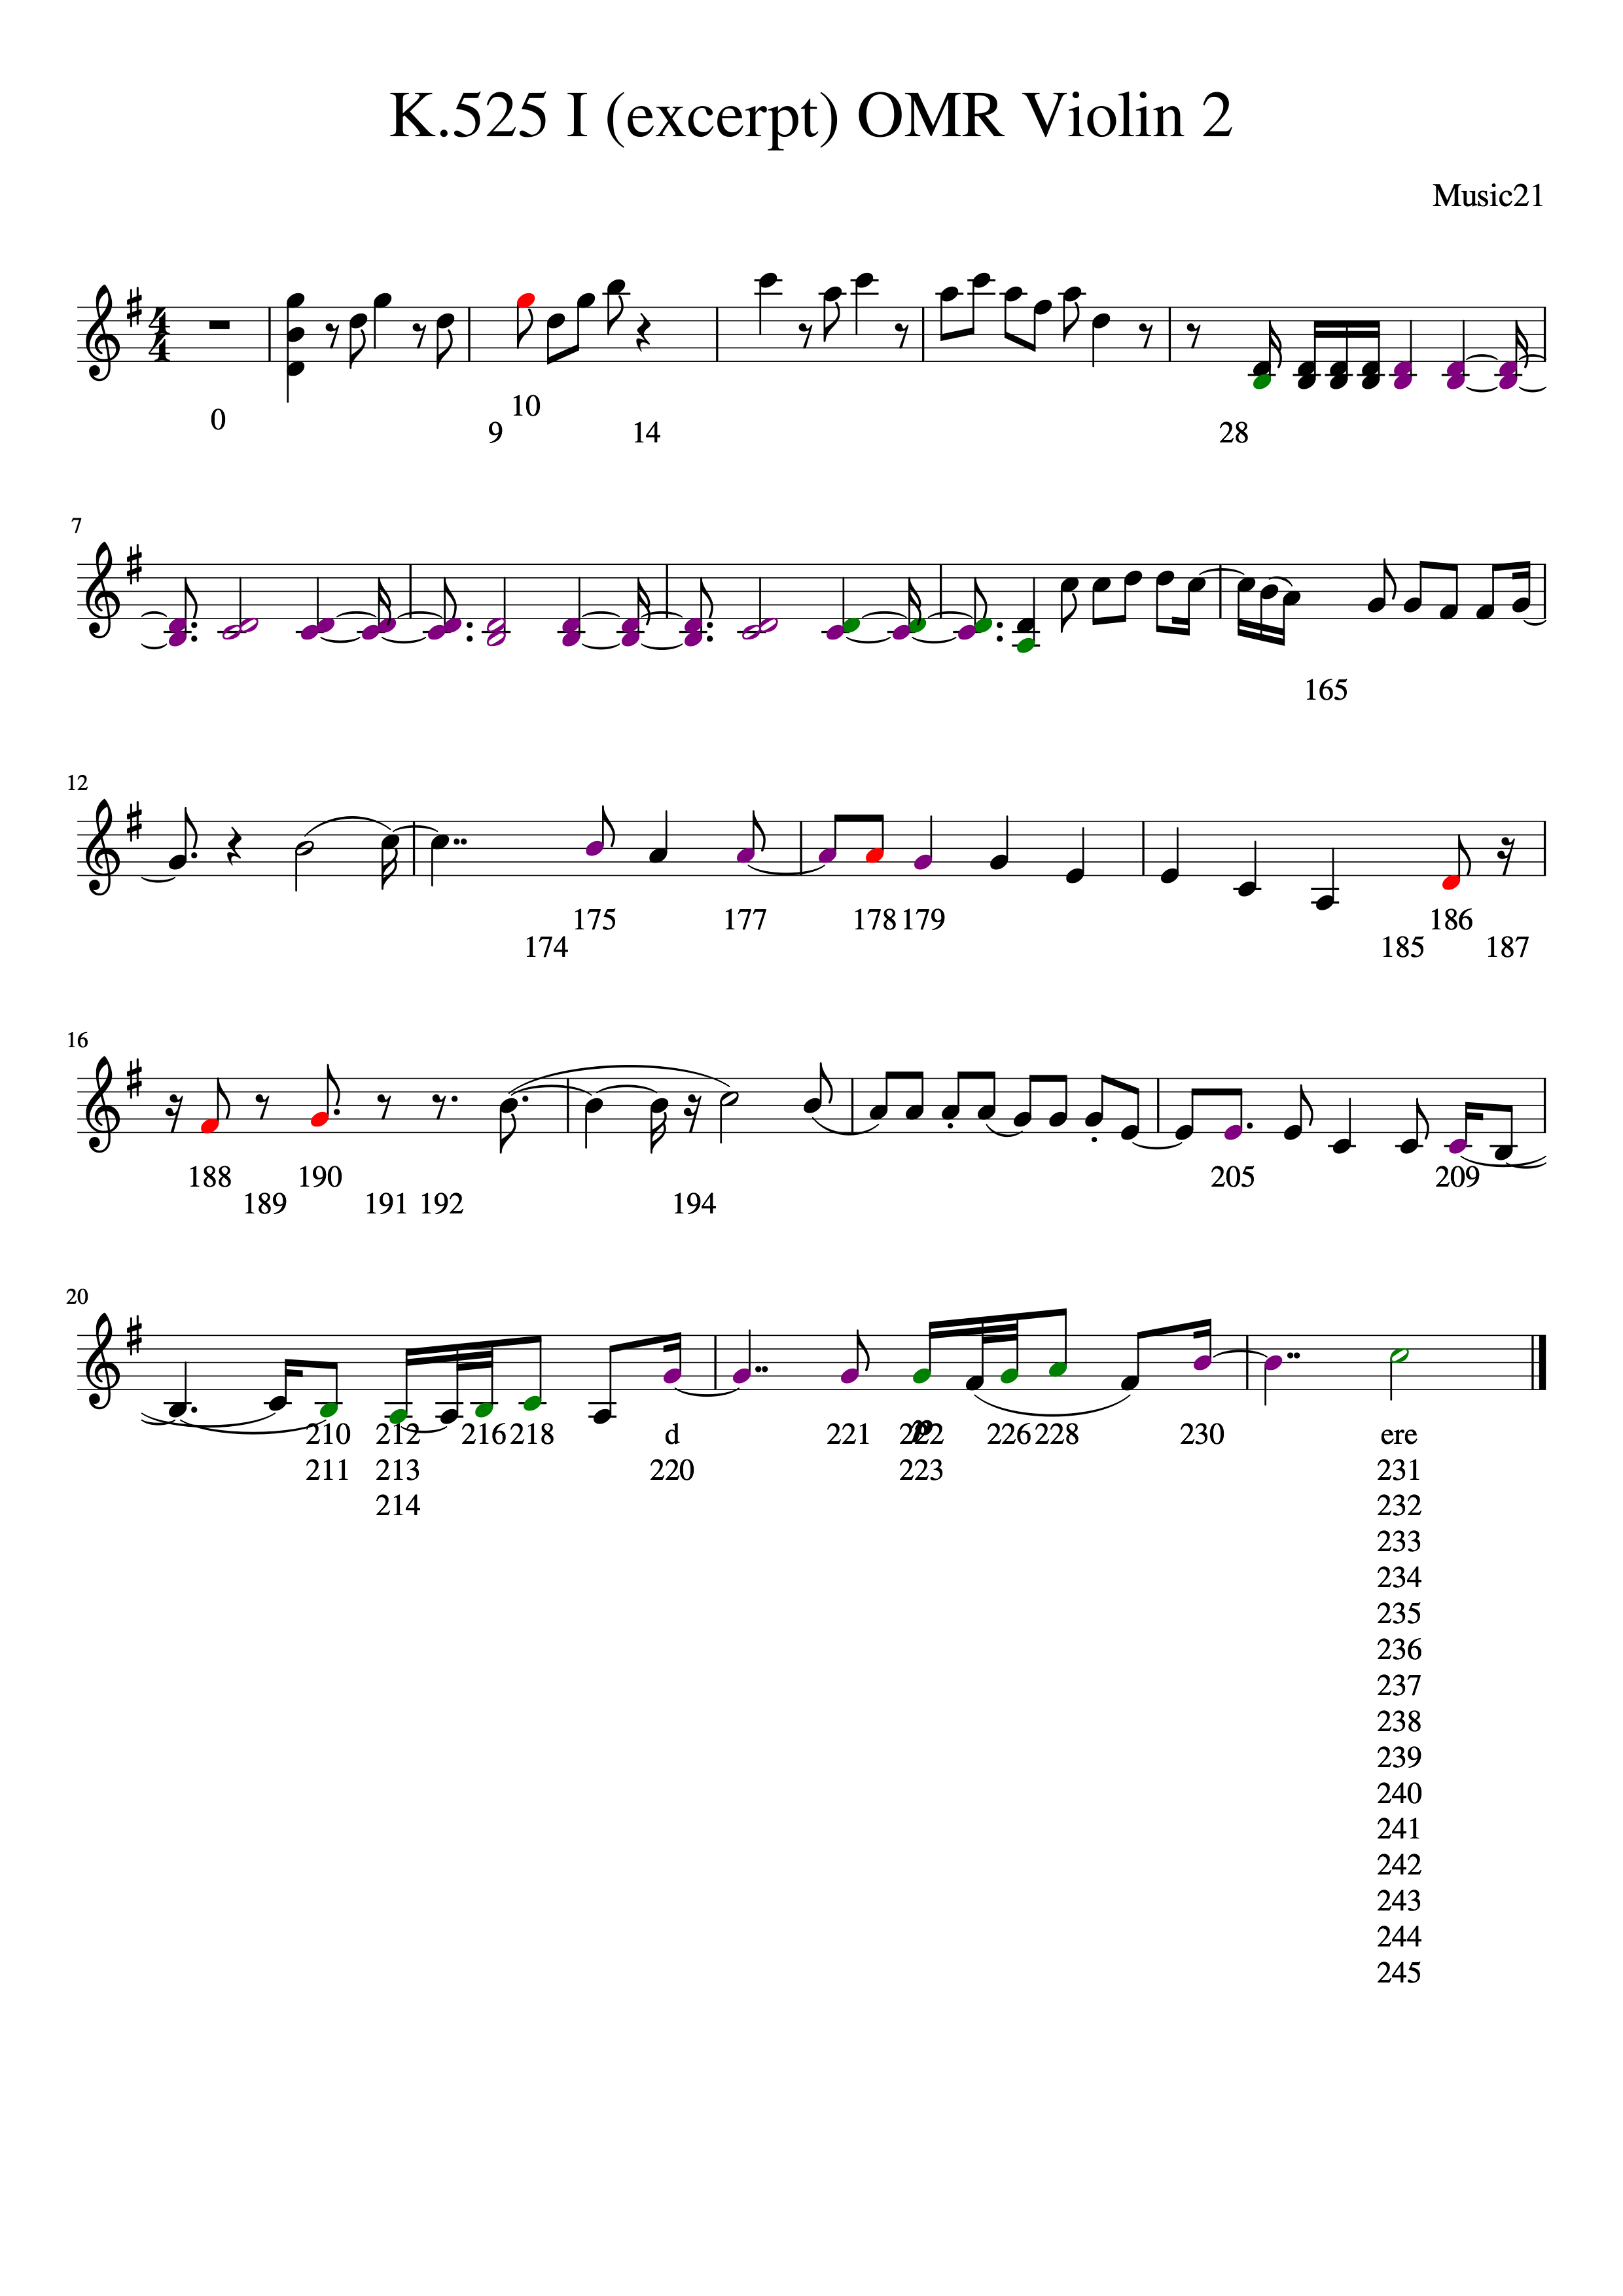
\includegraphics[width =.95\textwidth]{K525_I_OMR_Violin_2-1}
\caption{Visual display of changes in the Violin 1 part of source (OMR) stream.}
\end{figure}

Since this method has a lot of overhead, it is by default set not to run. It can be set to run for every alignment by passing in the argument \texttt{show=True}. 

\section{Fixer} \label{fixer}
The \texttt{Fixer} is the last part of the OMR/MIDI music stream alignment and correction system. Its developmental work can be found in \texttt{fixer.py}. There is a base class called \texttt{OMRMidiFixer} that takes as input the \texttt{changes} list that the \texttt{StreamAligners} outputs, as well as the original OMR and MIDI Streams.

Currently, there are two child classes, \texttt{EnharmonicFixer} and \texttt{DeleteFixer} that inherit from \texttt{OMRMidiFixer} and provide different fixing services. 

The \texttt{EnharmonicFixer} corrects a very specific type of error that appears in OMR, classified by Byrd as a pitch error \cite{byrd-testbed}. What happens in this scenario is that the MIDI score has the correct absolute pitch of a note, but might be spelled enharmonically, due to the fact that MIDI does not encode key signatures. The OMR score has been scanned incorrectly--- a sharp is mistaken for a natural or vice versa. An emergent property of this scenario is that the OMR note and the MIDI note could be on different lines or spaces but probably no more than a few steps apart. The \texttt{EnharmonicFixer} accounts for the various possibilities that arise in this situation and corrects the pitch of the OMR note by transposing the note 1 or 2 half steps and by adding or removing accidentals.

The \texttt{DeleteFixer} was designed to fit the specifications of the OpenScore project \cite{openscore}. The goal of the OpenScore project is to open-source music with open source software (like \texttt{music21}!). OpenScore will use a combination of computer and human power to digitize classical music scores and put them in the public domain. One idea is that software can identify wrong recognized notes in a scanned score and mark or delete the entire measure that that note is in and pass it off to a human corrector to re-transcribe the entire measure. The \texttt{DeleteFixer} could be the computer power in this method of score correction that OpenScore is using.

Any additional child Fixer classes would inherit from the parent \texttt{OMRMIDIFixer} class and also correct very specific problems. For example, in the \texttt{StaccatoFixer} skeleton code, would look for a specific pattern in the \texttt{changes} list that would indicate that the OMR process failed to recognize a passage that is marked as staccato. The \texttt{StaccatoFixer} class along with other children \texttt{Fixer} classes would look for similar patterns in the \texttt{ChangeTuples} list and correct the OMR stream based on this information. 

\section{Tradeoffs and Design Decisions}

In this section, I will justify some of my design choices and discuss tradeoffs in my decisions. 

\subsection{Modularity vs. Simplicity}
\subsubsection{A Variety of Settings and a Longer Setup}
All of the modules have many different settings with various parameters. The variety of settings is what makes the \texttt{Hasher} and \texttt{Aligner} so powerful--- by changing just a couple of settings, both are able to solve very different problems.

However, this necessarily lends itself to the system being more complex because each module must be able to handle various combinations of settings and their edge cases. It also requires the user to be careful when selecting initial settings. 

One alleviation to this problem is providing default settings to all the modules. These default settings are what I believe are good general settings for the most common uses of the modules. 

\subsubsection{Length Agnosticism}
There are two instances in which I purposefully built the system to be able to handle variable length input--- in building \texttt{NoteHash} and \texttt{NoteHashWithReference} tuples and in building the \texttt{OMRMIDICorrector} to be able to process a stream with any number of parts. Both of these decisions make the entire system more powerful because the system is able to process many more different types of streams this way, but it also makes the hashing and aligning process more convoluted. Fortunately for the user, all of this is hidden under the hood. There are likely some performance hits that are associated with this added complexity, but not to the point of inoperability. More demonstrations on timing are shown in section \ref{timing}.

\subsection{Performance vs. Space and Object Overhead}

\subsubsection{NoteHashWithReference}
The \texttt{NoteHashWithReference} object contains a reference to the original stream object. Streams and their elements are complex objects, so \texttt{NoteHashWithReference} objects have much more overhead in storage than their counterparts, \texttt{NoteHash} objects. However, in setting up a \texttt{Hasher} object, the user has the decision to use either one.   

\subsubsection{Creating One Hasher and Many Aligners}
During the correction process, only a single \texttt{Hasher} object is created and used and reused to generate hashes for every part in the stream passed in. There was the option of having \texttt{Hasher} object be one-time-use objects, but I chose to have the \texttt{Hasher} be able to operate on multiple streams. 

On the other hand, a new \texttt{StreamAligner} object is generated for every pair of parts in the OMR and MIDI streams that are passed in. 

Between generating \texttt{NoteHashWithReference} objects for every hashed stream element and \texttt{StreamAligner} objects for every pair of streams, there is a lot of space overhead taken up in even just a single alignment and correction process. However, based on experimental findings in which I tried to create these objects in C, perform the comparisons in C, and then translate the results into Python, I concluded that the limiting factor of the process was not in Pythonic object creation but rather the comparison process that calculates Levenshtein edit distance. The results and findings are discussed in more detail in section \ref{spaceoptimizations}.


\subsection{Manual User Input}
The OMR and MIDI streams that are used as input to the system come from somewhere. I have left the onus on the user to source .mid files and find scanned scores. I also have left it to the user to use some kind of OMR tool to convert the scanned score and the MIDI file into a musicXML form. Once in musicXML form, the user can use the \texttt{music21} library to parse the OMR and MIDI and convert them into \texttt{music21} streams. 

I leave this as a task to the user instead of automating it because with practice, humans can be much more precise and efficient with this process, and the necessity of a (probably large and complicated) computer program to do the same thing decreases. 
